\documentclass[%
 reprint,
%superscriptaddress,
%groupedaddress,
%unsortedaddress,
%runinaddress,
%frontmatterverbose, 
%preprint,
%showpacs,preprintnumbers,
%nofootinbib,
%nobibnotes,
%bibnotes,
 amsmath,amssymb,
 aps,
 pra,
%prb,
%rmp,
%prstab,
%prstper,
%floatfix,
]{revtex4-1}

\usepackage{graphicx}% Include figure files
\usepackage{dcolumn}% Align table columns on decimal point
%\usepackage{bm}% bold math
\usepackage{fullpage}
\usepackage{epsfig}
\usepackage{amsmath}
\usepackage{amsfonts}
\usepackage{amssymb}
\usepackage{float}
\usepackage{pstricks}
\usepackage{cancel}
\usepackage{lipsum}
%\usepackage[nottoc,numbib]{tocbibind} %Uncomment for bibliography to be its own numbered section
\usepackage{units}
\usepackage{listings}

\graphicspath{{../plots/}}

\begin{document}

\preprint{APS/123-QED}

\title{\textbf{Lab Report: Compton Scattering} \\ \small{And Investigation of the Angular Dependence of the Scattering Probability for Photons}}
\author{Joshua LaBounty}
\author{Thomas Krahulik}
\affiliation{Stony Brook University --- PHY 445}

\date{\today}

\begin{abstract}
	In this experiment, we test the classical Thompson Formula (Eq. \ref{eq:thompson}) against the Klein-Nishina Formula (Eq. \ref{eq:kn}), its quantum mechanical counterpart. At small angles, the two formulae agree quite well, but at large $\theta$ we see a significant deviation. In order to accomplish this, we look at Compton Scattering of $\gamma$-ray photons produced from the decay of a $^{137}$Cs source. We measure the angular dependence of the scattering probability $d\sigma / d\Omega$ in Aluminum at multiple angles ranging from $0^\circ - 110^\circ$ using a NaI(Tl) scintillating detector. We will also use this phenomenon to measure the mass of the electron and compare the number of free electrons in two different media: Copper and Aluminum.
\end{abstract}
\maketitle

\section{Background and Review of Previous Work}

In the early 1920s, A. H. Compton, discovered something peculiar in his study of X-ray scattering. They found that the frequency (and thus the energy) of X-rays decreased after scattering off free electrons in a medium. This result is not consistent with the classical electromagnetic theory of light, as the magnitude of the electromagnetic field cannot be altered by the change in direction constituted by the scattering. However, by considering the concept of light quanta (photons), Compton was able to build a model of the interaction between the incident photons and electrons using conservation of energy and momentum. In particular, he derived a form of the following relation:
\begin{gather}\label{eq:energy_scatter}
	E_\gamma ' = \frac{E_\gamma}{1 + \frac{E_\gamma}{m_e c^2} (1 - \cos{\theta})}
\end{gather}
This relates the incident energy of the photon with its final energy and the scattering angle. This formula was seen as major evidence in favor of the theory of light quanta, and has been experimentally verified numerous times.

Another facet of Compton's work with X-rays is his examination of the scattering angle. He found that the theoretical scattering probability (which he expressed in terms of $I/I_0$ and we look at as $d\sigma / d\Omega$) was inconsistent with the Thompson prediction:
\begin{equation}\label{eq:thompson}
	\frac{d \sigma}{d \Omega}_{Th} = \frac{r_0^2}{2}(1+\cos^2{\theta})
\end{equation}
Instead he found that, once again, classical theory was inadequate for describing these quantum phenomena. It wasn't until 1928 that Klein and Nishina, using quantum electrodynamics, derived a formula which included not only quantum effects but also relativistic corrections:
\begin{gather}
	\frac{d \sigma}{d \Omega}_{KN} = \frac{r_0^2}{2} \frac{1 + \cos^2{\theta}}{[1 + \gamma(1 - \cos{\theta})]^2} \nonumber * ~~~~~~~~~~~~ \\
	\left[ 1 + \frac{\gamma^2(1 - \cos{\theta})^2}{(1 + \cos^2{\theta})(1+ \gamma(1 - \cos{\theta}))}\right] 
	\label{eq:kn}
\end{gather}
where $\gamma = h\nu / m_e c^2$. A comparison of these two equations can be seen in Figure \ref{KN_vs_Thompson_Theory}.

This particular experiment, and its results, are well documented in various literature.

\section{Experimental Setup}

The source of the $\gamma$-rays for this experiment is a $^{137}$Cs sample, measured to emit $300~\mu Ci$ of radiation in 1978 and now emitting only $116~\mu Ci$ due to its decay, completely encased in lead save for a small aperture. This aperture is in line with the $0^\circ$ line on our table. On the other end of this experiment we have a movable detector. This detector consists of a NaI(Tl) scintillating crystal permanently bonded to a photomultiplier and a pre-amplifier. This detector is mounted on a movable platform which pivots around a point on the $0^\circ$ axis. Marks on the table allow us to rotate the detector semi-precisely about this axis to arbitrary angles. Also on this pivot is a mounting point for our scatterers, which consist of Aluminum and Copper cylinders with a hole drilled directly in the center. With the scatterer in place, the $\gamma$-rays which are emitted by the $^{137}$Cs pass through the aperture, scatter off electrons in the Al or Cu cylinders, and then pass into the NaI(Tl) crystal. These $\gamma$-rays produce scintillation photons proportional to their energy in the NaI(Tl) scintillation crystal. These scintillation photons are picked up as an electric signal by the photomultiplier, and then through two levels of amplification before being output to the Multi-Channel Analyzer (MCA). The MCA reconstructs the energy of the incident $\gamma$-rays from the signals and plots a histogram of Numbers of Photons detected vs. Bin Number (where the Bin Number corresponds to an photon energy). From there, the information is saved in a format which can be read into our data analysis software, ROOT. A diagram of this setup, taken from \cite{manual}, can be seen in Figure \ref{Setup} below:
\begin{figure}[H]
	\centering
	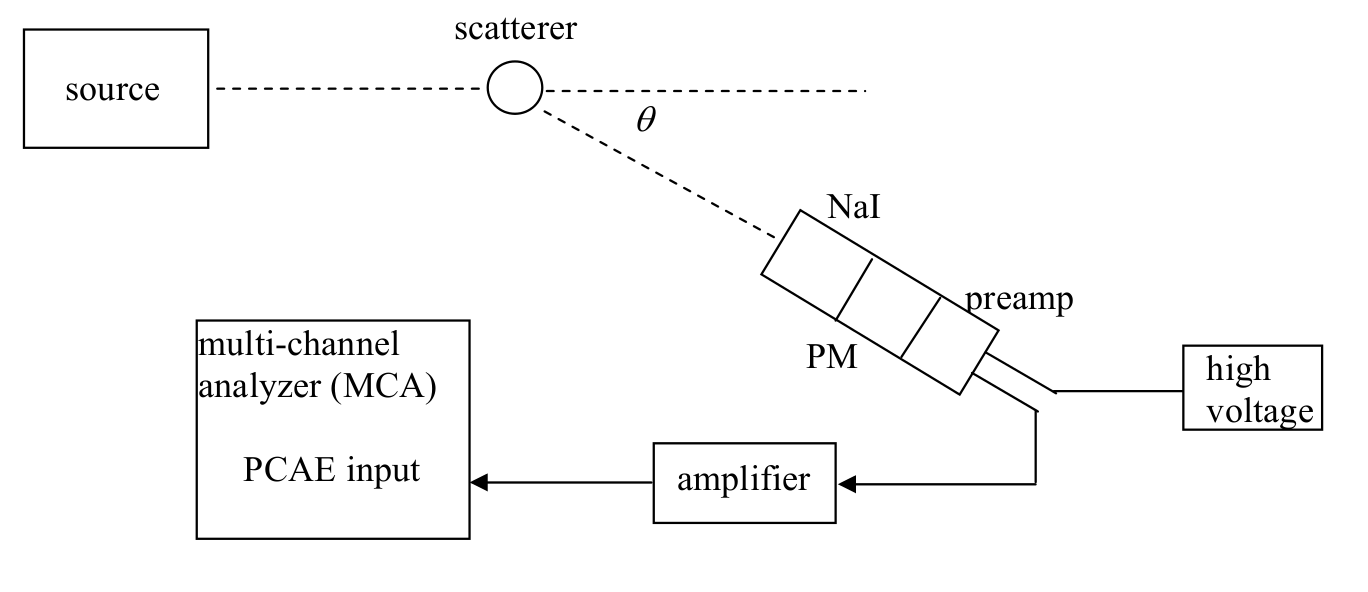
\includegraphics[width=0.4\textwidth]{Setup.png}
	\caption{Experimental Setup}
	\label{Setup}
\end{figure}

\section{Measurements}

\subsection{Calibration of Detector Energy Scale}
Before the gamma ray scattering from $^{137}Cs$ can be analyzed an energy calibration of the MCA program is required. This is done through analysis of the histograms generated by the data provided by the program. As previously mentioned, the MCA program stores a count of the events in each channel which can be plotted as a histogram. The peaks on such a histogram indicate the more frequent energies of photons emitted by the source. These peaks can be fit to a Gaussian function (sometimes with a background function) to find the mean value of the peak and a standard deviation. For many different sources, the mean value of these peaks can be identified as an energy value known to be characteristic of the spectrum of the source. As an example, the peak of the $^{137}Cs$ spectrum fitted in Fig.\ref{Fig:CsUncalib} is associated with an energy value of 661.6 keV. Fig.\ref{Fig:Na511Fit} demonstrates another example, with a fit of the 511 keV peak associated with electron-positron annihilation.
\begin{figure}[H]
\centering	
	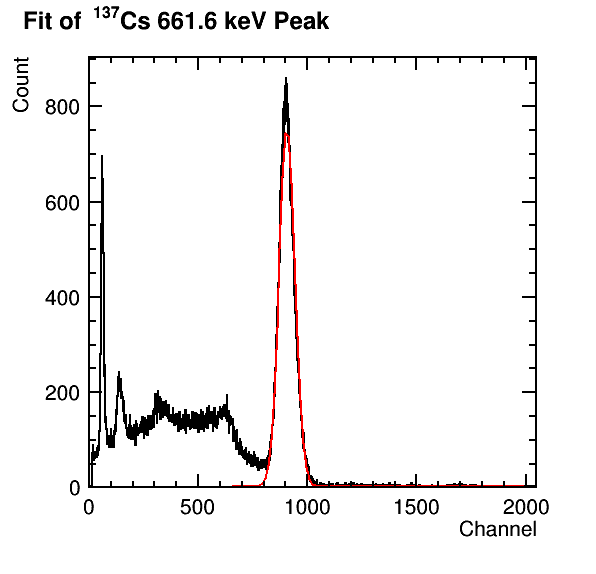
\includegraphics[width=0.4\textwidth]{Cs662keVFit.png}
	\caption{Fit of 661.6 keV Peak on $^{137}Cs$ Spectrum using Gaussian Function and a Background Exponential Decay}
	\label{Fig:CsUncalib}
\end{figure}

\begin{figure}[H]
\centering	
	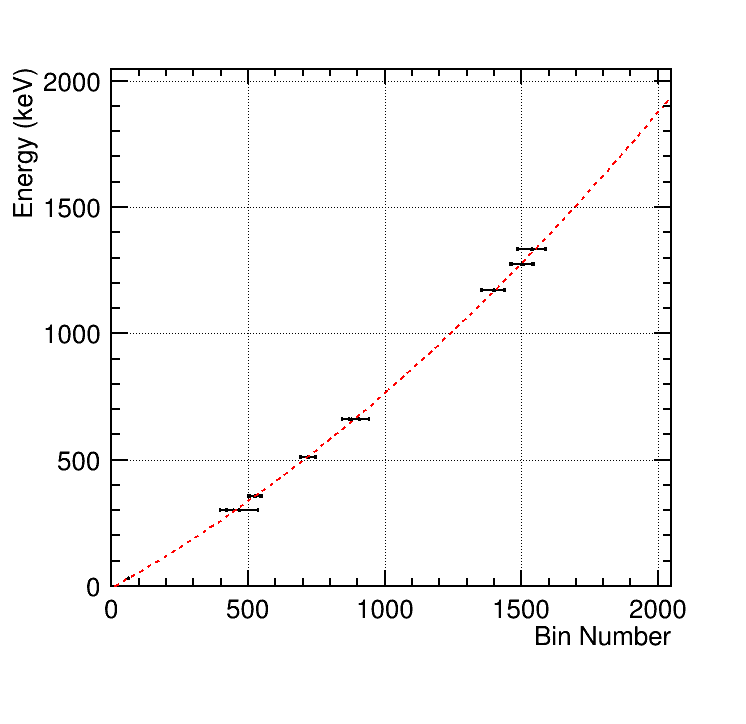
\includegraphics[width=0.4\textwidth]{BinvEnergy.png}
	\caption{Energy vs Bin Calibration Plot}
	\label{Fig:EvBin}
\end{figure}

\subsection{Electron Mass}

\subsection{Angular Dependence of the Scattering Probability}

\begin{gather}\label{eq:fitfunction}
	f(x) = [0]*e^{\frac{(x-[1])^2}{2*[2]^2}} + e^{[3]+[4]x} + [5]
\end{gather} 

After calibrating our detector and using that calibration to determine the electron mass, we sought to understand the angular dependence of the scattering probability for our $\gamma$-rays, or how $d \sigma / d \Omega$ changes with $\theta$. In order to do this, we placed the large Al scatterer at the pivot point of our setup and took spectra of the strong $^{137}$Cs. We measured the spectra, multiple times, at a number of angles between $0^{\circ}$ and $110^{\circ}$. At each angle, we fit the $661.6~keV$ peak to Equation \ref{eq:fitfunction} and integrated over the gaussian portion. This integral gives us our value for $Y(\theta)$. \textbf{Using the procedure outlined in \cite{milissinos}, we were able to identify values for $N_e$,$~ N_\gamma$,$~ \epsilon$, and $ d\Omega$ as well, which allowed us to solve for our experimental value of $d \sigma / d \Omega$.} We plotted this experimental value in Figure \ref{KN}.

\begin{figure}[H]
	\centering
	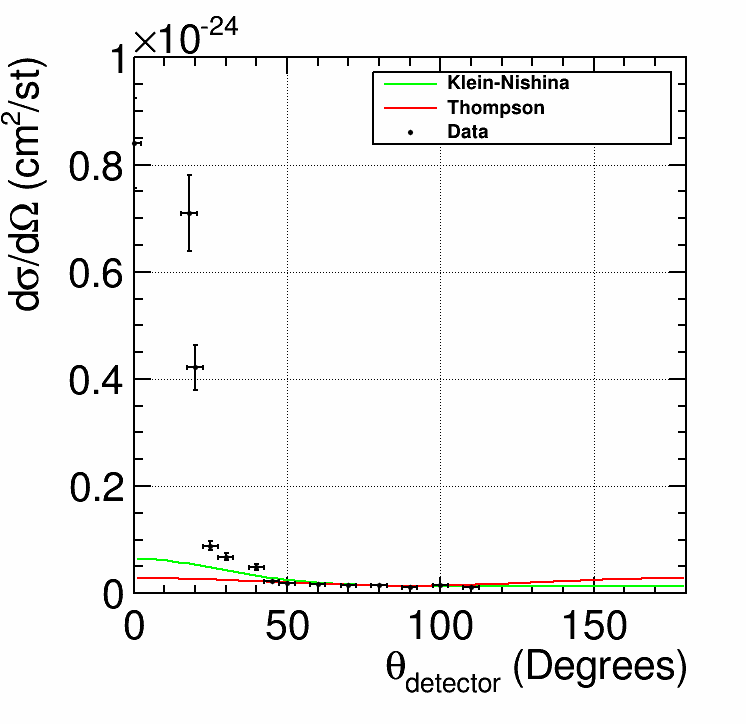
\includegraphics[width=0.4\textwidth]{KNvsThompson_Fit.png}
	\caption{Data from experimental measurement of $d\sigma/d\Omega$.}
	\label{KN}
\end{figure}

\noindent In the coming sections, we will compare this data to the results predicted by both the Thompson and the Klein-Nishina Formulae

\subsection{Free Electrons in Cu and Al}

\section{Theoretical Model}

\begin{figure}[H]
	\centering
	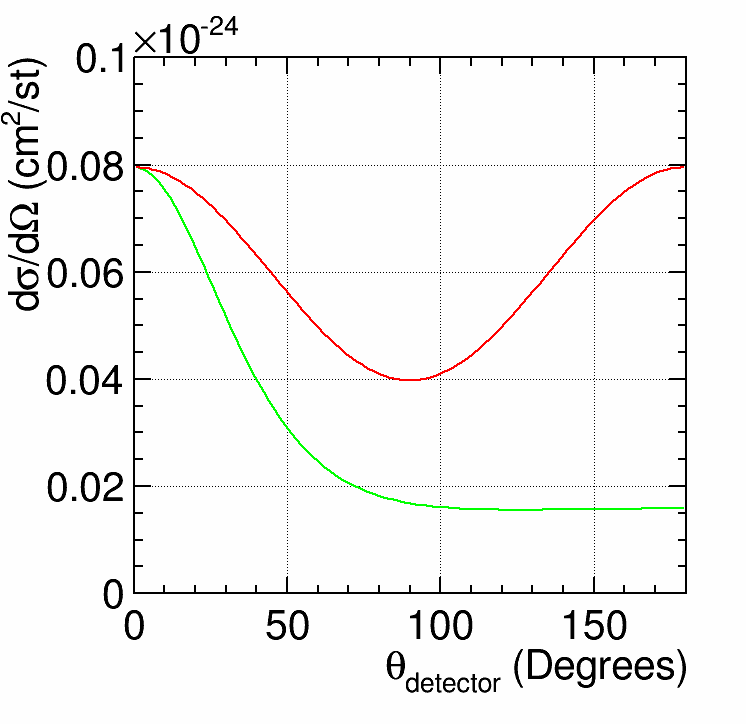
\includegraphics[width=0.4\textwidth]{KNvsThompson_TheoryOnly.png}
	\caption{Comparison of the Theoretical Predictions for the KN and Thompson Models}
	\label{KN_vs_Thompson_Theory}
\end{figure}

\subsection{Angular Dependence of the Scattering Probability}

\section{Comparison of Theory and Experiment}

\section{Discussion and Conclusions}

\section{Author Contributions}

\begin{thebibliography}{5}
	
	\bibitem{milissinos}
	A.C. Melissinos, Experiments in Modern Physics (Academic Press, NY, 1966).
	
	\bibitem{bevington}
	Philip R. Bevington and D. Keith Robinson, Data Reduction and Error Analysis 3rd edition (McGraw-Hill, 2003).

	\bibitem{bartlett}
	A. A. Bartlett, Am. J. Phys. 32 , 120 (1964).
	
	\bibitem{compton_paper_original}
	A. H. Compton, Phys. Rev. 21 , 483 and 715 (1923).
	
	\bibitem{manual}
	R. Lefferts, Compton Scattering (2010).


\end{thebibliography}

\begin{appendix}

\section{Derivation of Equation \ref{eq:energy_scatter}}

\begin{figure}[H]
	\centering
	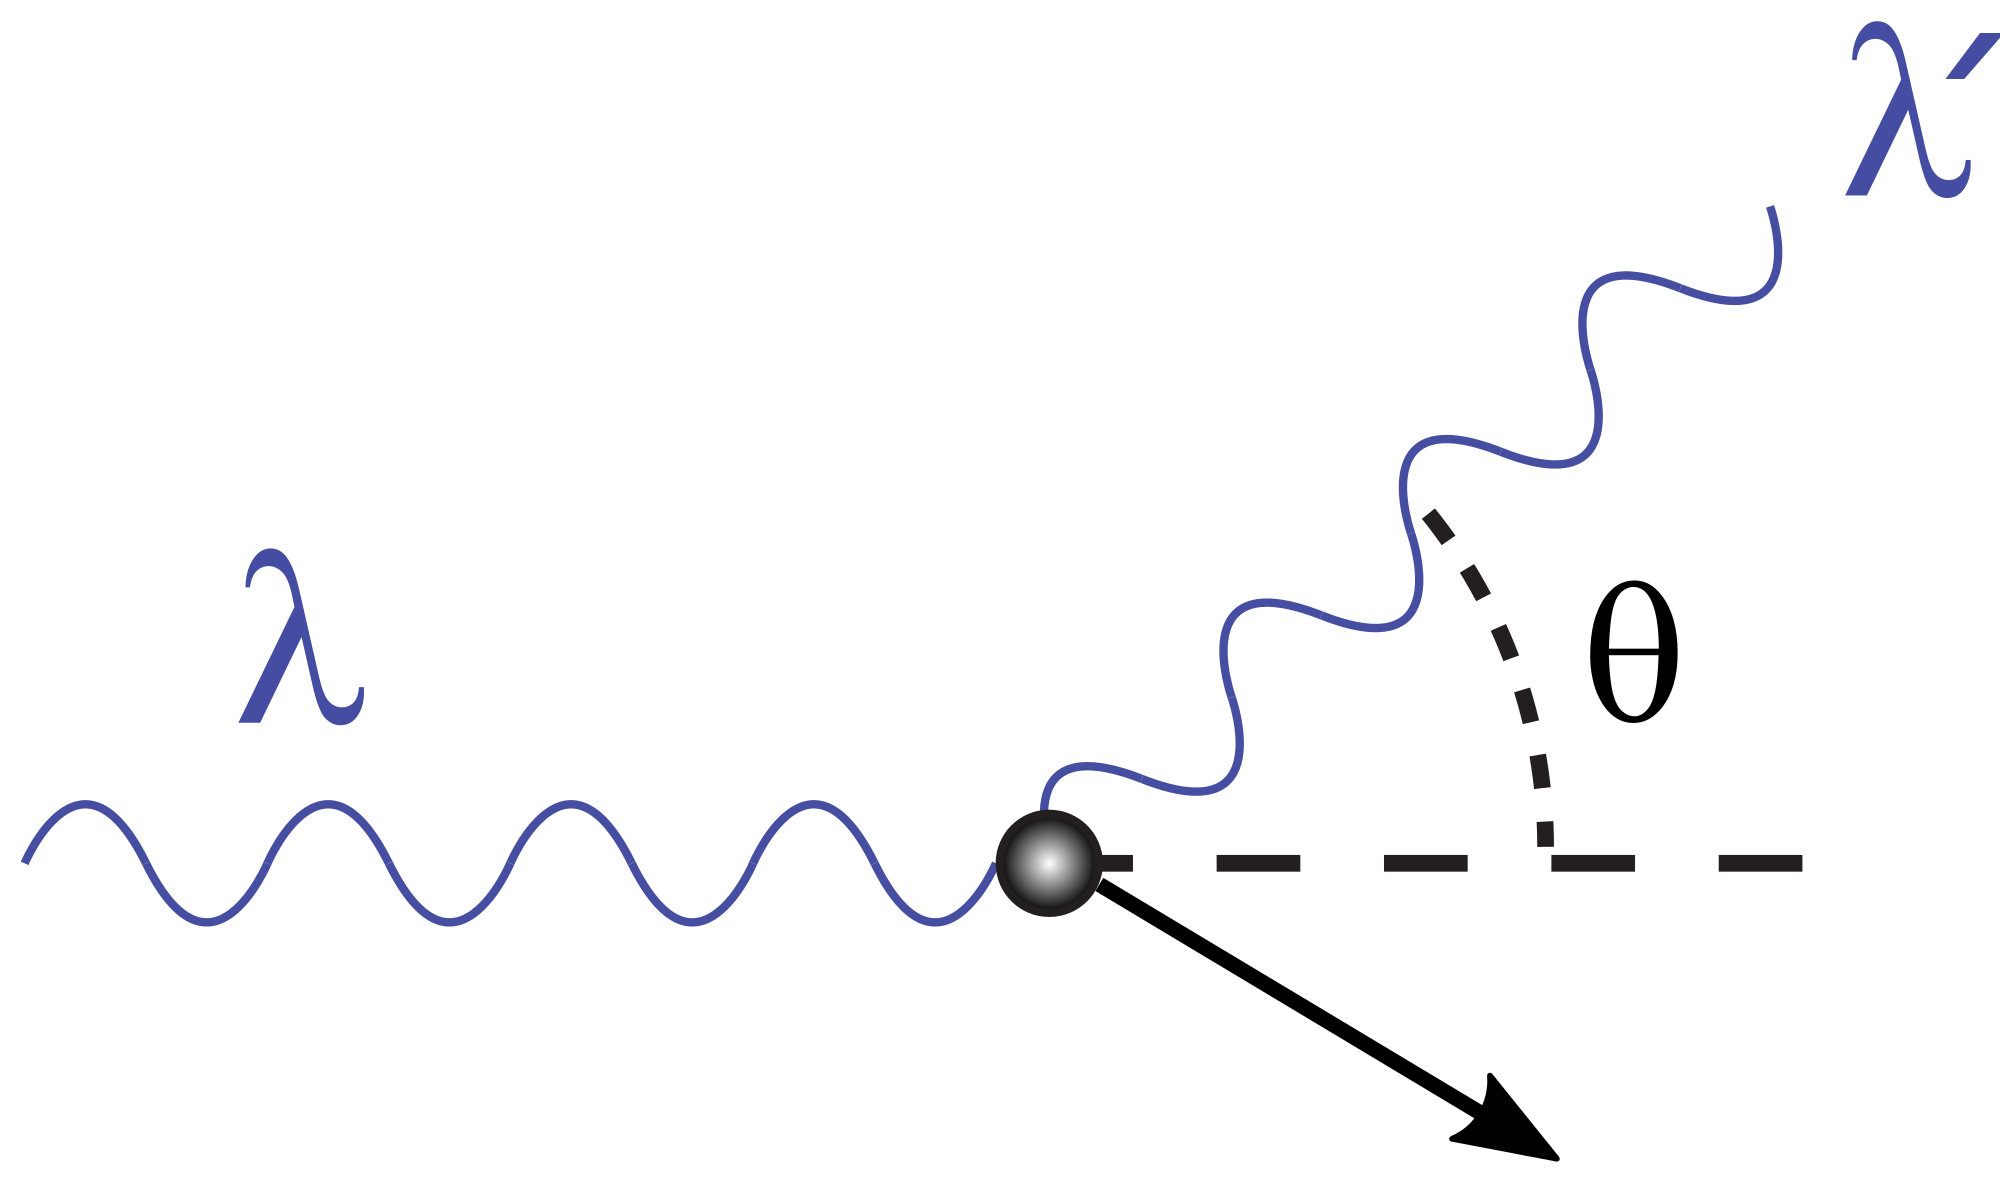
\includegraphics[width=0.3\textwidth]{../plots/ComptonDiagram.png}
	\caption{Diagram showing a photon scattering off an electron at rest. Image courtesy of Wikipedia.}
\end{figure}

This formula can be described semi-classically using only conservation of energy and conservation of momentum. We approximate this interaction as a photon impacting an electron which is currently at rest. The conservation laws require that:

\begin{gather}
	E_\gamma + E_e = E_\gamma ' + E_e '\nonumber \\
	\mathbf{p}_\gamma = \mathbf{p}_\gamma' + \mathbf{p}_e' \nonumber
\end{gather}
Initially:
\begin{gather}
	E_e = m_e c^2 \nonumber
\end{gather}
And after the collision:
\begin{gather}
	E_e' = \sqrt{(\mathbf{p}_e' c)^2 + (m_e c^2)^2} \nonumber
\end{gather}
Substituting these quantities into conservation of energy, we find:
\begin{gather}
	E_\gamma + m_e c^2 = E_\gamma' + \sqrt{(\mathbf{p}_e' c)^2 + (m_e c^2)^2} \nonumber \\
	\downarrow \nonumber \\
	\mathbf{p}_e^{2'} c^2  = (E_\gamma - E_\gamma' + m_e c^2)^2 - m_e^2 c^4 \nonumber
\end{gather}
Now returning to conservation of momentum:
\begin{gather}
	\mathbf{p}_e' = \mathbf{p}_\gamma - \mathbf{p}_\gamma' \nonumber
\end{gather}
Since these momenta are vector quantities, and we are only interested in a scalar, we can take the dot product:
\begin{gather}
	p_e^{2'} = \mathbf{p}_e' \cdot \mathbf{p}_e' = p_\gamma^2 + p_\gamma^{2'} - 2 p_\gamma p_\gamma' \cos{\theta} \nonumber \\
	p_e^{2'} c^2 =  p_\gamma^2 c^2 + p_\gamma^{2'} c^2 - 2 c^2 p_\gamma p_\gamma' \cos{\theta} \nonumber \\
	p_e^{2'} c^2 = E_\gamma^2 + E_\gamma^{2'} - 2 E_\gamma E_\gamma' \cos{\theta} \nonumber
\end{gather}
We can now equate these two equations for $p_e^{2'} c^2$ and find:
\begin{gather}
	(E_\gamma - E_\gamma' + m_e c^2)^2 - m_e^2 c^4 = E_\gamma^2 + E_\gamma^{2'} - 2 E_\gamma E_\gamma' \cos{\theta} \nonumber
\end{gather}
We then complete the square and reduce this equation in order to find:
\begin{gather}
	2 m_e c^2 (E_\gamma - E_\gamma') = 2 E_\gamma E_\gamma' (1- \cos{\theta}) \nonumber
\end{gather}
Which we rearrange to arrive back at Equation \ref{eq:energy_scatter}:
\begin{gather}
	E_\gamma ' = \frac{E_\gamma}{1 + \frac{E_\gamma}{m_e c^2} (1 - \cos{\theta})} \nonumber
\end{gather}
Compton's original formulation of this equation is just another form of this equation, rearranging some terms and substituting $\lambda$ for $E_\gamma$ using the relation $E_\gamma = hc/\lambda$.
\begin{gather}
	\lambda' = \lambda + \frac{h}{m_e c} (1 - \cos{\theta}) \nonumber
\end{gather}

\end{appendix}

\end{document}


































